%%% LearnPAd Document template / example using learnpad.cls class for styling
%%% 20140401, 
%%% Guglielmo De Angelis <guglielmo.deangelis@isti.cnr.it>
%%% Andrea Polini <andrea.polini@unicam.it>

\documentclass{learnpad}
% \usepackage{labsedc}
\usepackage[showtodos,showcomments]{labsedc}
\let\cleardoublepage\clearpage
\usepackage{extracommands}

%%% ------------------------------------------------------
%%% ---------------- The Title
%%% ------------------------------------------------------
\title{Integration plan} 

%%% ------------------------------------------------------
%%% ---------------- The Sub-Title
%%% ------------------------------------------------------
% \subtitle{} 

%%% ------------------------------------------------------
%%% ---------------- The Name of the Deliverable
%%% ------------------------------------------------------
\deliverableno{D7.1}

%%% ------------------------------------------------------
%%% ---------------- The Authors
%%% ------------------------------------------------------
\authors{Amira Ben Hamida (LIN), Vedran Hrgovcic (BOC), Fabio Mancinelli (XWIKI), Darius Silingas (NME), Jean Simard (XWIKI)}

%%% ------------------------------------------------------
%%% ---------------- The Editors
%%% ------------------------------------------------------
\editors{Vedran Hrgovcic (BOC)}

%%% ------------------------------------------------------
%%% ---------------- The reviewers
%%% ------------------------------------------------------
\reviewers{Amira Ben Hamida (LIN)} 

%%% ------------------------------------------------------
%%% ---------------- The date
%%% ------------------------------------------------------
\date{\today}

%%% ------------------------------------------------------
%%% ---------------- deliverable info
%%% ---------------- choose among : Report / Other / Prototype
%%% ------------------------------------------------------
\naturedeliverable{Report}%
%%% ------------------------------------------------------
%%% ---------------- deliverable dissemination levele
%%% ---------------- choose among the two options below:
\disseminationlevelpublic
% \disseminationlevelconfidential
%%% ------------------------------------------------------
\version{0.2}%
\contractualdeliverydate{31 July 2014}%
\actualdeliverydate{31 July 2014}%
\contributingwp{WP7}%

%%% ------------------------------------------------------
%%% ---------------- abstract
%%% ------------------------------------------------------
\abstract{\dots~\dots\TODO{TBD}}

%%% ------------------------------------------------------
%%% ---------------- Keywords
%%% ------------------------------------------------------
\keywords{\dots~\dots\TODO{TBD}}

%%% ------------------------------------------------------
%%% ---------------- review table
%%% ------------------------------------------------------
\reviewoutline{5 Jun 2014}{0.2}{N.A.}{N.A.}
\reviewdraft{text1}{text2}{text3}{text4}
\reviewqa{text1}{text2}{text3}{text4}
\reviewptc{text1}{text2}{text3}{text4}

\begin{document}

\frontmatter
\maketitle

%% ------------------------------------------------------
%% ---------------- document history
%% ------------------------------------------------------
\begin{history}
  \historyitem{0.1}{First ToC}{Vedran Hrgovcic, Fabio Mancinelli} 
  \historyitem{0.2}{Switch to the \LaTeX Template}{Jean Simard} 
\end{history}

%%% ------------------------------------------------------
%%% ---------------- review table with the previous info
%%% ------------------------------------------------------
\reviewtable

%%% ------------------------------------------------------
%%% ---------------- acronyms
%%% ------------------------------------------------------
\begin{acronyms}
  \acronym{CA}{Consortium Agreement}%
  \acronym{DL}{Deliverable Leader}%
  \acronym{DOW}{Description of Work}%
  \acronym{IAC}{Industrial Advisory Committee}%
  \acronym{MST}{Management support team}%
  \acronym{OSS}{Open Source Software}%
  \acronym{PL}{Project Leader}%
  \acronym{PMB}{Project Management Board}%
  \acronym{PO}{Project Officer}%
  \acronym{PTC}{Project Technical Committee}%
  \acronym{SL}{Scientific Leader}%
  \acronym{TL}{Technical Leader}%
  \acronym{WP}{Work Package}%
  \acronym{WPL}{Work Package Leader}%
  \acronym{CA}{Consortium Agreement}%
  \acronym{IAC}{Industrial Advisory Committee}%
\end{acronyms}

\tableofcontents

%%% ------------------------------------------------------
% In case you don't need one of the following list 
% just comment the line
%%% ------------------------------------------------------

%\listoftables 
\listoffigures 
%\listoflistings

%%% ------------------------------------------------------

\mainmatter

\chapter{Introduction}
\label{ch:introduction}

\section{Goal of this deliverable}
\label{sec:goal-of-this-deliverable}

The goal of this deliverable is to document every development and integration practice we agree
into the consortium in order to facilitate the development process between partners.
Since we want to offer maximum freedom in the choice of technologies of each component, this
deliverable will mainly focus on the tools and processes that will ease the collaboration like
source repositories, bug tracking system, documentation, continuous integration.

\section{Structure of the deliverable}
\label{sec:structure-of-the-deliverable}

In the Section~\ref{ch:preamble}, we will justify the choice of an SOA architecture for our
\learnpad platform and discuss the general choices related to open sources and closed sources
development. Section~\ref{ch:development-components} will be a general view of the development
process, from the first lines of codes to the publication of a stable version with all the
transitional steps. Section~\ref{ch:development-process} will develop and detail each of these
transitional steps, mainly in term of practices with some example of technical solutions to support
them. The integration plan will be detailed in section~\ref{ch:integration-plan}.

\chapter{Preamble}
\label{ch:preamble}

\section{SOA architecture}
\label{sec:soa-architecture}

The \learnpad project involves 9 partners, each of whom will produce one or more functionalities
in this architecture. To ease the collaboration between partners, we need to delimit the scope
for each functionality in order to precisely define the interactions needed. A solution to manage
this problem is encaspulation of functionalities which delimits the scope with inputs and outputs.
Encapsulation as services leads us to a \emph{Service-Oriented Architecture} also known as SOA.

SOA is a loosely coupled architecture which means that:
\begin{itemize}
	\item each service delimits a scope of functionalities
	\item each interaction between services is defined as a public interface
\end{itemize}

\section{Source management}
\label{sec:source-management2}

In \learnpad projects, most developments will be distributed under an Open Source license.
All source code developed in the consortium will be available publicly on a source versioning
system such as GitHub. Integration of proprietary products into the project where the source
is not available will be handled on a case by case basis.

\subsection{External service}
\label{sec:external-service}

In some cases, functionality can be deployed as a public service, accessible from any internet
connection (for example, REST API). In this case, the service can be developed independantly of
the main \learnpad platform and no file of any kind would be pushed on the source repository.
The development of this service would meet the requirements of a pre-defined roadmap and the
service must be available during test procedures.

\subsection{Internal service}
\label{sec:internal-service}

In cases when it is easier to create the service as a component inside of the \learnpad platform
(for example: a library or an executable), only the resulting binary file will be uploaded to the
public source repository. The development of this component can be independant of the main
development effort but it will still need to meet the requirements of a pre-defined roadmap.

\chapter{Development components}
\label{ch:development-components}

\section{Development workflow}
\label{sec:development-workflow}

\begin{figure}
\centering
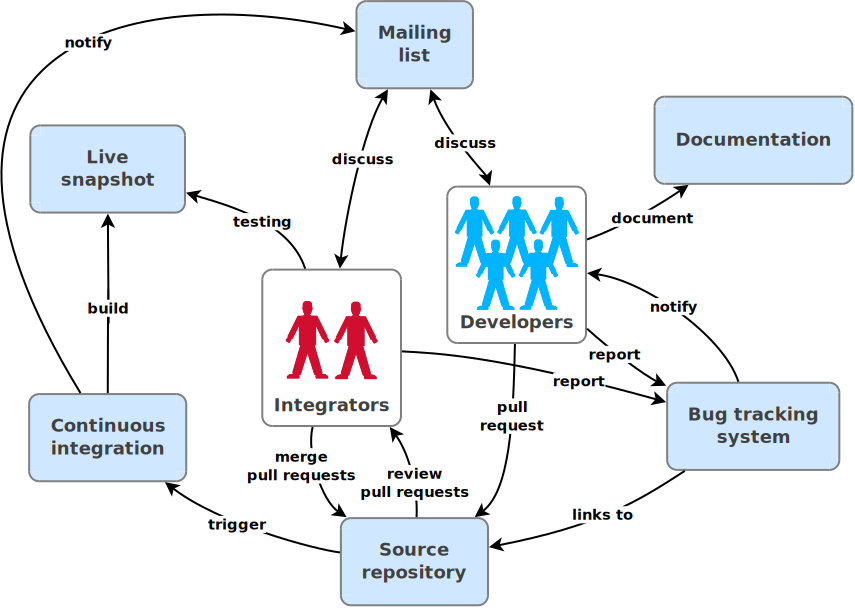
\includegraphics[width=0.67\textwidth]{images/development-workflow.png}
\caption{Development workflow with all tools}
\label{fig:development-workflow}
\end{figure}

\section{Details}
\label{sec:details}

The Figure~\ref{fig:development-workflow} illustrates the global development workflow.
In this workflow, there will be developers and integrators who interact using a variety of tools.
We will now give more details on these tools and how they will be used.

\subsection{Mailing list}
\label{sec:mailing-list}

An email mailing list will be available for general decision making about the platform,
the goal being to keep records of discussions and choices about developments or architecture design.

\subsection{Source repository}
\label{sec:source-repository}

A distributed source code repository will be provided for storing the source code or binaries
needed for building the \learnpad platform. The main repository will be stored in a public GitHub,
repository. Github is a popular code hosting and collaborative software development environment
which is free to non-private projects. Github provides not only a place to store the code but also
a rich variety of tools such as issue tracking, ability to browse code and readme files in a web
browser, advanced email notification, and well documented applications for all popular computer
Operating Systems.

Each developers will work on his own copy (or \emph{fork}) of the repository and propose new
functionality or bug fixes using Github \emph{pull requests}\footnote{A pull request is a method of
submitting contributions to a software project. It contains the \emph{patch} representing changes to
be made and creates a central place for those changes to be reviewed and discussed} which
integrators will have the duty to review. An integrator may accept the \emph{pull request},
request changes or further information or in an extreme case, close it pending further discussion.

Despite having direct access to the shared repository, an integrator who is also a developer should
make sure to use \emph{pull requests} for integrating their own functionality so as to allow for
discussion with other integrators and developers and to keep record of the contribution.

All developers should adopt the \emph{check in early and often} development methodology.
Code in development is not expected to be bug-free but great importance is placed on collaboration
and working in the open. In a fast-changing collaborative software development project, frequent
pull requests help everybody. They help the developer making them because he is able to avoid
rewriting code to cope with changes in other elements of the system and they also help other
developers who are able to see and adapt to changes in this developer's component.

\subsection{Documentation}
\label{sec:documentation}

An XWiki instance has already been provided and is currently being used for collaboration and
documentation. Documentation may accompanying the source code in the
repository or it may be placed on the wiki as long as relevant documents are referenced from the
source repository. The main entry point into the documentation for each partner's sub-folder will
be a file called \texttt{readme.md} (see Section~\ref{sec:source-structure} for more information
about partner sub-folders).

\subsection{Bug tracking system}
\label{sec:bug tracking-system}

All participants will be responsible for the discovery and diagnosis of bugs. Bugs, feature
requests, \emph{pull requests} and other to-do items shall be submitted to the Github bug tracking
system where others can keep track of issues which need to be addressed. Email notifications of new
issues will be sent to integrators and updates of an issue will be sent to those who participate in
(e.g. comment on) the issue.

\subsection{Continuous Integration Server}
\label{sec:ci-server}

Continuous integration will be provided by travis-ci, a hosted, distributed continuous integration
service used to build and test projects hosted at GitHub. Like Github, travis-ci service is free
for public projects and travis-ci provides email notification of build failures and GitHub
integration for automatically testing \emph{pull requests} before they are merged.
The Operating System on travis-ci build machines is Ubuntu Linux 12.04 LTS\footnote{The stable
version of a widely used Linux distribution.} which will heretofore be referred to as the
\emph{target system}, all parts of the online platform will be expected to build and run on this
system. Travis-ci is also capable of uploading and downloading files from other servers as part of
the build.

\chapter{Development process}
\label{ch:development-process}

\section{Documentation}
\label{sec:documentation2}

There are a few occasions when documentation will be needed such as architectural
design and configuration.

\subsection{Architecture design}
\label{sec:architecture-design}

According to the Agile Development Methodology, architectural design should not be set in
stone and changes can be made as experience is gained. Therefor architectural design
decisions need not be perfect the first time, better to have something quickly which
satisfies the obvious use cases than to try to project every possible need.

Discussion of architectural design should take place on the mailing list or in logged
chatroom where there is a record of the thoughts and reasoning. As ideas solidify and
consensus forms, they should move to the wiki where they become official documentation.

For producing diagrams, a server is available for collaborative work using MagicDraw.
When applicable, MagicDraw can be used for development of ideas on concert with the
mailing list. To minimize the number of places where documentation resides, ideas and
diagrams which have solidified should be exported and placed in the wiki or in the source
repository.

\subsection{Interfaces}
\label{sec:interfaces}

Two main types of interfaces are Application Programming Interface (API): the way in
which components communicate, and User Interface (UI): the way in which a component
communicates with a human. In either case it is important to clearly document interfaces
and put a link to this documentation in the \texttt{readme.md} file
(see Section~\ref{sec:source-structure}).
For UI development, use of mockups is highly recommended.

\subsection{Configuration and Deployment}
\label{sec:deployment-process}

Since the system will be automatically installed on a live test server
(see Section~\ref{sec:live-snapshot}), each component requiring configuration must contain
default configuration.

Documentation of the configuration should be done in the configuration files. If more
documentation is necessary, there must be URLs in the configuration file which tell
administrators where to find the additional information.

\section{Roadmap and Development Milestones}
\label{sec:roadmap}

There is two different types of roadmaps.

\subsection{Global roadmap}
\label{sec:global-roadmap}

The global roadmap will be a broad picture of the project, based on the deliverable
deadlines. Releases will take place every three months or six Development Milestones.
In the final two week period before the release date, the most recent Development
Milestone will be manually tested by each partner in order to verify that the
features for which this partner is responsible work well. At the beginning of this
two week development cycle, a stable branch will be created and only critical and
"safe" bug fixes will be accepted to the branch prior to release.

\subsection{Partner roadmaps}
\label{sec:partner-roadmaps}

Each component will have a responsible partner and this partner must provide a roadmap
detailing timeframes and objectives for the components under their responsibility. At any
given time, a roadmap should contain goals for the next three months.
Development Milestones will take place every two weeks and each two weeks there will be
a roadmap meeting to check in on progress and set new goals. Each partner's roadmap
should be contained in a document on the wiki where it can be reviewed at each bi-weekly
roadmap meeting.

\section{Source management}
\label{sec:source-management}

All source code will be stored in a single repository using a distributed version control
system such as git. To simplify collaboration, each component will be developed in one
sub-folder of a \texttt{components} directory. The source will be published on a public
server such as GitHub, where it can be cloned or viewed with a web browser.

\subsection{Source structure}
\label{sec:source-structure}
The partner in charge of managing development of a component will be free to organize the content
of this sub-folder in any way as long as a few standardized files are contained within.

\begin{itemize}
\item \texttt{readme.md} This file will contain the entry-point to all documentation of this
component. At the very least, this file must contain contact information for the manager of
the component and a link to their roadmap (see: Section~\ref{sec:roadmap}).
\item \texttt{build} This will be a script file which is executable on the \emph{target system}
(see Section~\ref{sec:continuous-integration}) and will build the component.
\item \texttt{builddeps.txt} This \emph{optional} file will contain a list of packages which
need to be installed using the \emph{target system's} package manager (EG: apt-get) in order for
the component to be built.
\item \texttt{out} This folder will be created by the \emph{build} script and will contain the
result of the build, everything that is necessary for this component to run.
\item \texttt{out/etc} This folder, named after the UNIX \texttt{/etc} configuration folder will
contain all of the configuration files necessary for the component.
\item \texttt{out/start} This will be a script file which initiates the completed component, it will
expect it's configuration to reside in the \emph{out/etc} folder and must be capable of starting
the component with no manual intervention.
\item \texttt{out/stop} This script will behave similarly to \emph{start} but will stop the running
component.
\item \texttt{out/rundeps.txt} This \emph{optional} file will contain a list of package names,
like \texttt{builddeps.txt}, but with packages necessary for the component to \emph{run}.
\end{itemize}

\subsection{Source development flow}
\label{sec:source-development-flow}

We will use the \emph{git flow}\cite{kreeftmeijer:2010} development model. The main repository will
contain a \texttt{master} and a \texttt{develop} branch. Every developer should work on his
own fork of the project then submit pull requests (see Section~\ref{sec:source-repository})
which will be checked by integrators for merging with the \texttt{develop} branch of the main
repository. Then, for each Development Milestone or release, the \texttt{develop} branch will
be merged onto the \texttt{master} branch. Thus the \texttt{master} branch will always contain
the most recent Development Milestone version.

\section{Building}
\label{sec:building}

As seen in the Figure~\ref{fig:development-workflow}, a continuous integration will support the
development of the platform. That means that every service must be automatically buildable.
As seen in Source Management (see Section~\ref{sec:source-management}), each service will be a
folder in the source repository in order to maximize freedom in the management of development
activities (tools used, subdirectories, etc.). To simplify the overall build, each folder must
contain a standardized script for building the component in that folder how that script manages
the build is an implementation detail.

At the root of the repository, a global builder will parse all of the services to build them.
If specific deployment procedures must be done, they should also appear in this build process.

\section{Testing}
\label{sec:testing}

Unit tests may be run as part of the build process but integration tests which require the
\learnpad platform in a running state must be handled differently. The exact methodology
remains a topic for further research but possible solutions include a special sub-folder
for all integration tests or a set of integration tests included in each component and built
separately from the normal build.

\chapter{Integration plan}
\label{ch:integration-plan}

\subsection{Continuous integration}
\label{sec:continuous-integration}

Continuous integration is an automated process by which the current state of the source code is
built into a final product, any automated tests are run and the final product is made available
to developers so that they can test the interaction of their commits in near-real-time. The platform
will be built and deployed on the \emph{target system}, a computer running an installation of
Ubuntu 12.04 LTS \footnote{The stable version of a widely used Linux distribution.}.
Automated builds may also be used as an aid for integrators to do "smoke test" validation on pull
requests before accepting them. In order to protect the working environment of all developers,
it is critical that integrators reject or revert any pull request which causes an incorrect build
of the platform.

\subsection{Live snapshot}
\label{sec:live-snapshot}

Periodically, the most recent build of the \learnpad platform will be automatically published
on a live server running the \emph{target system} so that it can be accessible to all of the
collaborators. This will aid in bug detection and provide a base for discussion of additional
features and the direction of the project.

\subsection{Release Process}
\label{sec:release-process}

As described in the Global Roadmap (see Section~\ref{sec:global-roadmap}), releases will happen
every 6 Development Milestones. In the final 2 week development cycle before the release, a stable
branch of the source code will be created and partners will be asked to test the features for
which they are responsible. The live snapshot will be available for this. During these two weeks,
only minor bug-fix patches will be accepted to the stable branch and only if Integrators judge them
to be low risk to the release. At the end of the 2 week development cycle, a final version of the
release will be created and made available for download by the partners and stakeholders.


% ---------------------------------- Bibliography starts here
% ----------------------------------

\bibliographystyle{plain} 
\bibliography{biblio}

\end{document}
